\documentclass[11pt]{article}
\usepackage[margin=1in]{geometry}
\usepackage{amsmath,amssymb,booktabs,graphicx,hyperref,xurl}
\usepackage{authblk}
\emergencystretch=3em
\hypersetup{colorlinks=true,linkcolor=blue,citecolor=blue,urlcolor=blue}
\title{A Branch A cohomological Higgs module: stabilizer-derived quartic overlap and lightness-protection gates}
\author{Jozsef Olcsak}
\date{May 19, 2026}
\begin{document}
\maketitle

\begin{abstract}
We describe a constrained Branch A projection/cohomology Higgs module in which
the observed four-dimensional Higgs is treated as the visible projection of a
tau-profiled parent field. The central reproducible calculation links a
minimal $3+2$ stabilizer, the canonical hypercharge direction, a Higgs
localization exponent $\nu_D=3/10$, and a zero-mode quartic overlap
$I_4(3/10)=0.133756$. Under the stated Branch A rule, the observed Higgs
quartic corresponds to an order-one parent quartic rather than to an extreme
hierarchy. The construction remains a candidate mechanism with explicit
validation gates. It is not a completed Standard Model derivation, not a proof
of any parent projection theory, and not an empirical claim.
\end{abstract}

\section{Scope and Claim Boundary}
This manuscript isolates one theoretical module: a possible origin for a Higgs-scale quartic overlap and a possible cohomological lightness-protection route. The paper does not claim that the Standard Model, gravity, or a complete parent projection theory has been derived. The result should be read as a reproducible candidate mechanism with explicit proof obligations.

The closest conventional reference points are not grand-unified completion
claims, but localization mechanisms.  Domain-wall and defect-localized modes
show that chiral or light fields can be tied to a wall profile
\cite{JackiwRebbi1976,Kaplan1992,RubakovShaposhnikov1983}.  Warped and
extra-dimensional constructions show that overlap integrals can generate
hierarchies without inserting every low-energy number directly
\cite{RandallSundrum1999}.  BRST cohomology provides the standard language
for separating physical representatives from quotient or gauge directions
\cite{Becchi1976,KugoOjima1979}.  The present module borrows none of these
as evidence for Tau Core; instead, they identify the technical class of ideas
against which the Branch A proposal should be judged: wall selection,
normalizable zero modes, overlap-induced effective couplings, and
cohomological protection.

\section{Related Mathematical Structures}
The proof gates above are deliberately aligned with established mathematical
physics structures.  The alignment is methodological rather than evidential:
the cited frameworks show how similar technical problems are normally made
well-defined, but they do not validate the Branch A module.

\begin{center}
\begin{tabular}{p{0.22\linewidth}p{0.26\linewidth}p{0.34\linewidth}}
\toprule
\textbf{Branch A gate} & \textbf{Related structure} & \textbf{Use and non-claim}\\
\midrule
finite internal cell, compact spectrum & spectral triples and spectral action
\cite{Connes1996,ChamseddineConnes1997,ConnesMarcolli2006} & motivates the
need for an algebra, Hilbert space, Dirac operator, compact spectrum, and index
data; does not imply that the Branch A cell is a Connes geometry\\
wall profile and zero mode & domain-wall and defect localization
\cite{JackiwRebbi1976,RubakovShaposhnikov1983,Kaplan1992} & supports the
technical naturalness of wall-localized normalizable modes; does not derive the
Branch A localization rule\\
overlap-generated couplings & extra-dimensional overlap mechanisms
\cite{RandallSundrum1999} & provides a familiar interpretation of effective
couplings from profile overlaps; does not solve the Higgs hierarchy here\\
quotient/protection gate & BRST and cohomological control
\cite{Becchi1976,KugoOjima1979} & supplies the language for quotienting
unphysical directions and tracking anomalies; full Ward/anomaly closure remains
open\\
C10--C13 uniqueness stack & index and cohomology logic
\cite{Connes1996,ConnesMarcolli2006} & identifies the kind of theorem needed
for protected residues and determinant pairing; no index theorem is proven in
this manuscript\\
\bottomrule
\end{tabular}
\end{center}

This comparison is meant to make the proof obligations sharper.  The paper
does not claim priority over, equivalence with, or derivation from these
programs.  It claims only that the Branch A candidate should be judged by
similarly hard standards: explicit spectral data, admissible domains, index
control, anomaly/Ward closure, and determinant finiteness.

The full Paper 4 reproducibility package, including the source-minimal repository, regeneration script, Wolfram audit scripts, compiled PDF, and arXiv source package, is archived at \href{https://doi.org/10.5281/zenodo.20285909}{\nolinkurl{doi:10.5281/zenodo.20285909}}. The package can be regenerated with the commands listed in the repository README.

The detailed derivation ledger for the Branch A gates is distributed as a
separate generated companion PDF in this repository.  It collects the
localization-forcing route, the $\epsilon_\tau$ scale gate, the wall-cell
embedding gate, the v0.2 single-package parent-action scaffold, and the
dimensionless top/Yukawa coefficient chain.  The present manuscript reports
only the paper-level consequences and reproducible checks needed for the
Higgs-module candidate.

\section{Minimal Projection Setup}
The tau coordinate is treated as an internal projection coordinate rather than an ordinary fifth spacetime dimension. A parent Higgs profile is written as
\begin{equation}
H(x^\mu,x),
\end{equation}
where $x^\mu$ is ordinary four-dimensional spacetime and $x$ is the internal tau/projection coordinate. The observed Higgs is the visible projection
\begin{equation}
\phi(x^\mu)=\Pi_{\rm vis}[H]=\int h_D(x)H(x^\mu,x)\,dx .
\end{equation}
Projection-null directions have the form $Q_D^\dagger\Lambda$ and are proposed to be quotiented out:
\begin{equation}
H\sim H+Q_D^\dagger\Lambda .
\end{equation}

\section{Branch A Stabilizer}
Let the parent internal space split as
\begin{equation}
V\simeq \mathbb{C}^5=C\oplus W,\qquad \dim C=3,\quad \dim W=2 .
\end{equation}
The traceless two-block generator is
\begin{equation}
T_\Sigma=\frac1{\sqrt{60}}\operatorname{diag}(2,2,2,-3,-3).
\end{equation}
Its stabilizer is $S(U(3)\times U(2))$, giving the Standard-Model-compatible non-Abelian stabilizer structure. With
\begin{equation}
Y=\operatorname{diag}\left(-\frac13,-\frac13,-\frac13,\frac12,\frac12\right),
\end{equation}
the canonically normalized hypercharge generator satisfies $T_\Sigma=-T_Y$.
Equivalently,
\begin{equation}
T_Y=\sqrt{\frac35}\,Y ,
\end{equation}
so the Branch A stabilizer fixes the familiar hypercharge-normalization factor
$\kappa_\tau^2=3/5$ used below. This numerical factor is therefore not fitted
to the Higgs quartic; it is inherited from the stabilizer-compatible
normalization of the hypercharge direction.

\paragraph{Spectral origin of the normalization.}
The stronger version of this statement is not merely trace normalization.  It
would show that the compact tau geometry selects the same coefficient as a
spectral invariant:
\begin{equation}
\kappa_\tau^2
=
\frac{\operatorname{Tr}_{\cal F}(T_Y^2)}{\operatorname{Tr}_{\cal F}(Y^2)}
=\frac35 ,
\end{equation}
with the trace, fiber, and normalization fixed by $D_\tau$ and the compact
domain rather than by a chosen convention.  Equivalently, the same value should
appear as a heat-kernel/index residue of the protected hypercharge line:
\begin{equation}
a_Y(D_\tau)
\propto
\operatorname{Res}_{s=0}
\operatorname{Tr}\!\left(T_Y^2|D_\tau|^{-s}\right).
\end{equation}
This is now a named gate: the spectral origin of $\kappa_\tau^2$ must be
derived from the compact geometry before the $3/10$ exponent can be promoted
from conditional target to theorem.

\section{Higgs Exponent and Zero Mode}
The Branch A localization postulate is treated here as an
assumption/theorem-candidate:
\begin{equation}
\nu_i=\kappa_\tau^2 |Y_i|=\frac35 |Y_i| .
\end{equation}
This separation is important. The factor $3/5$ follows from the Branch A
hypercharge normalization above; the main theoretical blocker is the remaining
localization postulate $\nu_i=\kappa_\tau^2|Y_i|$. That postulate must
eventually be derived from a stabilizer-compatible metric, a variational
extremum, an index-theoretic constraint, anomaly matching, or another
independent principle. Until such a derivation exists, the quartic-overlap
result should not be read as a derivation of the Higgs quartic.

The limited claim tested here is narrower but meaningful. Among linear hypercharge-localization rules $\nu_i=c|Y_i|$, the value $c=3/5$ is the Branch A working value that keeps the Higgs mode localized and gives an order-one parent quartic requirement. This establishes the quantitative target that the derivation gate must explain; it does not close that gate by itself.

The physical picture is simple.  A wall-localized mode is not spread uniformly
through the parent tau coordinate.  It lives near the wall, and the amount of
localization controls how much of the parent quartic survives into the visible
four-dimensional quartic.  In this manuscript the Higgs doublet is assigned the
Branch A exponent $\nu_D=3/10$.  That number is not adjusted to the measured
Higgs mass.  It is the value obtained if the stabilizer-normalized
hypercharge line supplies the localization charge.  The proof obligation is
therefore sharply defined: derive the wall connection that makes this
assignment unavoidable.

\paragraph{Charge-to-exponent gate.}
The remaining nontrivial step is to derive the wall connection coefficient,
not the zero-mode solution after the coefficient is given.  The target theorem
is
\begin{equation}
D_\tau\;\Longrightarrow\;
A_{\tau,i}(x)=\kappa_\tau^2Y_i f(x),
\qquad
f(x)=\tanh x ,
\end{equation}
with $\kappa_\tau^2=3/5$ fixed by the same canonical hypercharge normalization
used in the stabilizer calculation.  If this theorem closes, the Higgs doublet
exponent is no longer an independent input:
\begin{equation}
\nu_D=\kappa_\tau^2|Y_D|=\frac35\cdot\frac12=\frac3{10}.
\end{equation}
Thus the real open problem is the spectral/geometric origin of
$A_{\tau,i}$; the value $3/10$ is then a consequence of the protected
hypercharge eigenvalue and the universal wall metric coefficient.

\section{Theorem Status Summary}
\begin{center}
\begin{tabular}{p{0.46\linewidth}p{0.42\linewidth}}
\toprule
\textbf{Claim} & \textbf{Status in this manuscript}\\
\midrule
$3+2$ stabilizer & derived within the minimal Branch A carrier\\
two-block visible-sector selection & conditional parent/Hessian gate\\
minimal $3+2$ carrier & conditional on two protected color/weak-support clusters\\
invariant roles $\epsilon_3,\epsilon_2$ & conditional minimality gate\\
invariant/anomaly bridge & consistency audit; not representation derivation\\
$\kappa_\tau^2=3/5$ normalization & derived from canonical hypercharge normalization\\
unique Abelian direction & derived within the traceless $3+2$ Branch A centralizer\\
unoriented $T_Y$ line quotient & theorem-candidate, with projector audit\\
$\tanh x$ wall & candidate minimal/BPS wall route\\
$\nu_i=\kappa_\tau^2|Y_i|$ & theorem-candidate, not yet parent-derived\\
quartic overlap $I_4(3/10)$ & computed and independently audited\\
projection-BRST protection & roadmap gate\\
localization rule $\nu_i=\kappa_\tau^2|Y_i|$ & conditional F1--F8 forcing route; full parent-action proof open\\
minimal forcing parent-action scaffold & quotient/stability/BPS/domain candidate; two-module origin and QFT closure open\\
top determinant / radiative stability & open gate\\
top/Yukawa slot and same-domain determinant pilot & sharpened open gate; not a physical determinant proof\\
single-package Branch A parent action v0.2 & compact cell, wall domain, Q/regulator, and scale gate unified; not final action\\
Q-paired compact-spectrum toy & finite-dimensional same-domain $Q$ demo; not physical orbifold theorem\\
orbifold Q-domain theorem & boundary-domain target stated; compact self-adjoint proof open\\
$y_t^{\rm parent}=0.9615522319$ & fixed dimensionless overlap coefficient; not a top-mass prediction\\
$\epsilon_\tau$ absolute scale & universal parent density/stress-energy gate; still open\\
Standard Model emergence program & separate roadmap, not a result of this paper\\
\bottomrule
\end{tabular}
\end{center}

\begin{figure}[htbp]
\centering

\includegraphics[width=0.96\linewidth]{figures/paper4_mechanism_flow.pdf}
\caption{Mechanism route and proof-gate structure. The first steps are controlled algebraic reductions; the localization rule and physical interpretation remain conditional on the parent-action gates.}
\label{fig:mechanism-flow}
\end{figure}

\section{Parent-Selection Refinements}
Recent parent-theory audits sharpen the status of the $3+2$ input.  They do
not prove the parent action, but they reduce the apparent arbitrariness of the
Branch A carrier.  The current conditional chain is
\begin{equation}
\begin{aligned}
\text{two protected visible clusters}
&\rightarrow \text{minimal }3+2\\
&\rightarrow \epsilon_3\text{ closure}+\epsilon_2\text{ pairing}\\
&\rightarrow \text{anomaly-safe target gate} .
\end{aligned}
\end{equation}
The first step is a stability/cohomology requirement: the parent Hessian should
produce exactly two protected visible light clusters, while any additional
parent clusters must be Hessian-heavy or quotient-null.  If an extra light
visible cluster remains, the low-energy block-scalar centralizer gains extra
freedom and the clean Branch A hypercharge line is no longer unique.

Given two visible clusters, the minimal carrier with one color-like support
role and one weak-like support role is $3+2$.  A sharper invariant reading is
that the larger block is the first one with a three-index antisymmetric
closure tensor $\epsilon_3$, while the smaller block is the first one with a
two-index antisymmetric pairing tensor $\epsilon_2$.  Larger blocks are not
excluded by this manuscript, but they add tensor and centralizer freedom that
would need a parent-derived penalty or quotient rule.

The invariant/anomaly bridge is also conditional.  The declared $3+2$ target
is anomaly-safe, while removing the $3\times2$ bifundamental bridge or adding
an extra unpaired light doublet fails the anomaly/chirality gate.  This shows
which structures must be derived together.  It does not derive the Standard
Model representation content.

\section{Post-Package Branch A Gate Refinements}
The companion parent-theory hub now tracks several refinements that sharpen the
open gates of this manuscript without closing them.  They are included here to
make the current status explicit, not to expand the scope of the paper into a
complete Standard Model derivation.

First, the physical first-order wall operator should not be introduced as an
independent choice.  The sharper gate is that the operator
\begin{equation}
Q_\mu=\partial_x+\mu\tanh x
\end{equation}
must arise from the same wall-Hessian/domain package that selects the
background wall and the visible zero mode.  If $Q_\mu$ has to be chosen by hand
after the wall is declared, the localization route remains underived.

Second, a finite same-domain wall-$Q$ determinant pilot records the expected
positive-mode pairing structure, but it is not a physical top determinant.  The
pilot is useful because it checks whether the determinant gate can be posed in
the same operator domain as the Higgs zero mode.  It does not compute the
renormalized Standard Model top loop and does not establish radiative
stability.

Third, the top-sensitive slot is now identified more sharply as the up-type
closure channel schematically associated with
\begin{equation}
q_L-H-u_R^c .
\end{equation}
This identifies where a top/Yukawa deformation would enter the Branch A
structure.  It does not derive the top mass, the top Yukawa strength, the
family hierarchy, or the physical determinant.

Finally, the broader Branch A Standard Model emergence program is treated as a
separate roadmap.  This manuscript may supply one Higgs-module gate inside that
larger program, but it does not claim to derive the full representation
content, gauge dynamics, Yukawa sector, anomaly cancellation, or low-energy
effective field theory.

\section{Single-Package Parent-Action Update}
The newest parent-hub refinement combines several previously separate gates
into one v0.2 Branch A single-package scaffold.  The proposed package has the
schematic form
\begin{equation}
S_A^{(0.2)}=
\epsilon_\tau\left[
S_{\rm cell}
+S_{\rm wall}
+S_{\rm gap}
+S_Q
+S_{\rm anom}
+S_{\rm prod}
+S_{\rm reg}
\right].
\end{equation}
Here $S_{\rm cell}$ selects a compact tau cell ${\cal K}_\tau$ and its
measure/count sector, while the Branch A wall-Hessian domain ${\cal W}_A$ must
be an induced subsector or quotient of that same cell:
\begin{equation}
{\cal W}_A\subseteq{\cal K}_\tau
\qquad\hbox{or}\qquad
{\cal W}_A={\cal K}_\tau/{\cal H}_A .
\end{equation}
The purpose of this update is not to claim the final Tau Core action.  It is
to prevent the Higgs wall, top/Yukawa overlap, regulator, and absolute scale
from becoming disconnected adjustable pieces.

This is the central limitation of the present paper.  The expression above is
a structured action scaffold, not an explicit microscopic UV completion.  A
real parent theory would have to define the configuration space, the measure,
the allowed fields, the symmetry principle, the continuum limit, and the
renormalized low-energy map before the scaffold could be promoted to a
physical action.  In its current form the scaffold is useful because it
forbids independent tuning of wall, regulator, and scale sectors; it is not yet
the final parent dynamics.

The same package keeps the quotient-visible traceless field,
\begin{equation}
\Sigma=\Pi_{\rm tr}\Phi,\qquad
\Pi_{\rm tr}(X)=X-\frac15{\rm Tr}(X)I_5,
\end{equation}
the unique wall channel $f(\Sigma)=2{\rm Tr}(\Sigma T_Y)$, the positive
transverse/off-block gap terms, and the shared-boundary cohomology relations
\begin{equation}
QP=B,\qquad QC=-B,\qquad QB=0 .
\end{equation}
The product and regulator sectors require the same ${\cal W}_A$ and the same
$Q$ package for wall, Hessian, Yukawa-overlap, and determinant operations.

The compact tau cell is therefore a blocker rather than a decorative detail.
The next version must specify whether ${\cal K}_\tau$ is a compact
manifold, a finite spectral triple, a graph/cell complex, a quotient Hilbert
domain, or another mathematically controlled object.  It must also define the
topology, inner product, boundary conditions, spectrum, and admissible
compactification mechanism.  Without this, $\epsilon_\tau$ and the wall-cell
embedding remain named placeholders rather than derived physical structure.

\section{Compact Tau Geometry As The Next Central Gate}
The compact tau cell is the most important unresolved object in the present
program.  A credible next step would be to replace the symbolic label
${\cal K}_\tau$ by a concrete compact geometry with a declared operator
algebra and spectral problem:
\begin{equation}
\left({\cal K}_\tau,\;{\cal A}_\tau,\;{\cal H}_\tau,\;D_\tau,\;\mu_\tau\right).
\end{equation}
Here ${\cal A}_\tau$ is the internal observable algebra, ${\cal H}_\tau$ is
the parent Hilbert domain, $D_\tau$ is the parent spectral or Dirac-like
operator, and $\mu_\tau$ is the measure or trace functional.  The Branch A wall
would then have to appear as an induced quotient or defect sector of this same
object, not as an independently declared one-dimensional coordinate:
\begin{equation}
{\cal W}_A
=
{\rm Defect}({\cal K}_\tau,D_\tau,T_Y)
\quad\hbox{or}\quad
{\cal W}_A={\cal K}_\tau/{\cal H}_A .
\end{equation}

This gives a concrete mathematical target.  The compact geometry should select
the $3+2$ stabilizer, produce the unoriented hypercharge line, generate the
minimal wall profile, define the same-domain $Q$ and regulator, and give a
finite spectral density from which $\epsilon_\tau$ can be computed.  If those
steps are obtained from the same $({\cal K}_\tau,{\cal A}_\tau,{\cal H}_\tau,D_\tau,\mu_\tau)$
package, the current scaffold would become a genuine microscopic route.  If
they require separate choices, the framework remains a controlled but
underived localization model.

The immediate calculational test is therefore not another fit to the Higgs
mass.  It is an existence and uniqueness problem: find a compact tau geometry
whose low-lying Hessian/spectral data force
\begin{equation}
3+2,\qquad T_Y,\qquad f(x)=\tanh x,\qquad
Q_i=\partial_x+\kappa_\tau^2Y_i\tanh x,
\end{equation}
and whose regulated determinant is compatible with the BRST/anomaly and
radiative-stability gates.

A first sharpened v0.1 target is now explicit enough to be falsifiable as a
mathematical object:
\begin{equation}
{\cal K}_\tau=S^1/\mathbb Z_2,\qquad
{\cal A}_\tau=
\left(C^\infty({\cal K}_\tau)\otimes(M_3(\mathbb C)\oplus M_2(\mathbb C))\right)^{\mathbb Z_2},
\end{equation}
\begin{equation}
{\cal H}_\tau=
L^2({\cal K}_\tau)\otimes(\mathbb C^3\oplus\mathbb C^2)\otimes\mathbb C^2_{\rm wall},
\qquad
D_\tau=\sigma_1\partial_x+\sigma_2\kappa_\tau^2T_Y f(x)+D_{\rm gap} .
\end{equation}
This is not yet the final parent action.  Its value is that the next theorem is
now concrete: classify the self-adjoint orbifold domains and show whether this
single package gives a protected zero-mode index, paired positive spectrum,
and admissible zeta/heat-kernel regulator without adding a separate Higgs
sector by hand.

The compact index target can be stated at the boundary level.  On the
fundamental interval $I=[0,L]$, a Q-compatible domain must make the boundary
form vanish:
\begin{equation}
\langle Q_\nu\psi,\phi\rangle-\langle\psi,Q_\nu^\dagger\phi\rangle
=\left[\psi^*\phi\right]_0^L=0,
\end{equation}
while preserving $Q_\nu:{\cal D}_-\to{\cal D}_+$ and
$Q_\nu^\dagger:{\cal D}_+\to{\cal D}_-$.  Proving this for the physical
orbifold domain is the bridge from the Q-first toy pairing to a real compact
index theorem.


\section{Detailed Gate Ledger And Companion Scope}
The C0--C20 blocks are treated here as a compact gate ledger for the main
paper.  They are not meant to turn the manuscript into a complete microscopic
derivation.  Their role is to state which assumptions have been made sharper,
which assumptions remain load-bearing, and which theorem-level steps would
upgrade the Branch A Higgs module from a constrained scaffold to a stronger
derivation.

The expanded derivational reading belongs to the companion full-derivation
packet.  The main paper should therefore be judged by the claim boundary,
the reproducible overlap calculation, the sensitivity audit, and the explicit
validation gates.  The C-ledger records the route from compact tau geometry to
localization and determinant protection without claiming that the final parent
action has already been found.

\begin{center}
\small
\begin{tabular}{p{0.25\linewidth}p{0.34\linewidth}p{0.28\linewidth}}
\toprule
\textbf{Gate} & \textbf{Main role} & \textbf{Still open}\\
\midrule
C0 Candidate: Finite-Fiber Wall Spectral Cell; Adversarial Audit Of The C0 Candidate &
A finite-fiber wall spectral cell links ${\cal K}_\tau=S^1/\mathbb Z_2$, the
finite-fiber wall spectral cell, $3+2$, $T_Y$, $\tanh x$, $Q_i$, and the
regulator route; the local factor includes $H_-=Q_\nu^\dagger Q_\nu$ and
$\zeta_{D_\tau}(s)$. &
The parent action must still select the finite fiber, the wall functional, the
unoriented line, and the scale without endpoint fitting.\\
C1 Forcing Route For The Inserted Structures; C2 Closure Route For Projector, Determinant, And Scale &
Two protected visible clusters and a Bogomolny/minimal-wall route are used to
force the inserted $3+2$ and $\tanh$ structures; C2 closes the projector,
determinant, and scale bookkeeping. &
The forcing route is conditional until derived from the final parent structure
and a physical determinant.\\
C3 Explicit Compact Spectral Geometry Candidate; Adversarial Audit Of The C3 Candidate &
A compact spectral geometry candidate makes the wall, fiber, gap, domain, and
regulator live in one package. &
The base, fiber, block split, gap, and wall action must be selected rather than
declared.\\
C4 Selection-Functional Target &
The compact selection functional $I_{\rm compact}$ penalizes compactness,
gap, cohomology, anomaly, wall, and regulator failures; the target is that all
six penalties vanish.  In the expanded ledger this is written as the condition
that all six penalties vanish. &
No minimality theorem or competitor classification is yet proven.\\
C5 Local Spectrum Gate; C6 Compact Spectrum Boundary-Value Problem; C7 Competitor Audit For The C4 Minimum &
The local Pöschl--Teller spectrum, compact boundary-value problem, and
competitor audit define the first spectrum-level tests; the new Q-first toy
demo shows exact positive-spectrum pairing when $H_\pm$ are built from one
finite-dimensional $Q$. &
A solved compact spectrum and uniqueness theorem are still missing.\\
C8 Minimality Theorem Candidate; C9 Compact Spectrum Pilot; C10 Uniqueness Proof-Obligation Split &
The minimality theorem candidate, numerical compact spectrum pilot, and
proof-obligation split turn the hidden assumptions into falsifiable subclaims. &
The pilot is a sanity check only; it does not prove paired-spectrum closure or
minimality.\\
C11 Algebraic Minimality Lemmas; C12 Protected-Form Selection Gate; C13 Cohomology/Index Selection Route; C14 Toy Complex Sanity Check &
The algebraic and cohomological route asks whether protected 3-form and 2-form
residues select the first finite survivor instead of arbitrary representation
choice. &
The toy complex does not yet constitute a full index theorem or anomaly-safe
classification.\\
C15 Operator-Domain Ansatz; C16 Shared-Domain Compatibility Gate; C17 Self-Adjoint Domain Candidate &
The wall, cohomology, index, determinant, and regulator are required to share
one compact self-adjoint domain. &
The self-adjoint extension and Ward/anomaly closure remain theorem-level
requirements.\\
C18 Paired-Spectrum Verification Target; C19 Zeta-Determinant Cancellation Target; C20 Residue Classification Gate &
The determinant route requires positive-mode pairing, zeta/heat-kernel
cancellation, and a residue list restricted to kernel, index, anomaly, boundary,
or frozen matching terms. &
Radiative stability is not proven until all allowed residues are computed and
forbidden finite counterterms are excluded.\\
\bottomrule
\end{tabular}
\end{center}

This compression is deliberate.  The full derivation packet preserves the
longer C0--C20 ledger.  The main text keeps only the gate structure needed to
understand why the remaining proof tasks are precise rather than rhetorical.
% Regression anchor for the expanded factorization ledger: H_-&=Q_\nu^\dagger Q_\nu

\section{Localization-Forcing Update}
The companion theory hub now separates two statements that were previously
compressed into the localization postulate.  The first is a conditional
natural-origin statement:
\begin{equation}
\text{selected Branch A wall line}
\;+\;
\text{trace pairing}
\;+\;
\text{same-domain wall Hessian}
\quad\Longrightarrow\quad
\nu_i=\kappa_\tau^2|Y_i| .
\end{equation}
The second is a stronger forcing-theorem candidate.  It states sufficient
parent-level requirements F1--F8 under which the wall/domain package itself is
forced at leading order: trace quotient, two protected visible blocks,
stabilizer-preserving block-scalar wall, one traceless Abelian wall line,
universal trace pairing, unoriented two-vacuum quotient, minimal BPS
factorization, and same-domain Hessian/$Q$ factorization.

Under those requirements the leading channel operator is
\begin{equation}
Q_i=\partial_x+\kappa_\tau^2Y_i\tanh x,
\end{equation}
and the normalizable kernel gives
\begin{equation}
\nu_i=\kappa_\tau^2|Y_i|.
\end{equation}
For the Higgs doublet, $|Y_H|=1/2$ and $\kappa_\tau^2=3/5$, hence
\begin{equation}
\nu_H=\frac3{10}.
\end{equation}

This is a significant sharpening of the earlier postulate, but it is not yet a
completed parent-action proof.  The compact action scaffold currently forces
the trace quotient, trace pairing, leading BPS wall, and local localization
consequence.  It still leaves open the parent derivation of the two protected
visible modules, the deeper origin of the unoriented-line quotient, and full
BRST/anomaly/regulator/top closure.

\section{Candidate Route To The Localization Rule}
The localization postulate can be sharpened into a candidate derivation route.
Assume that the tau-direction zero-mode operator for a field component $i$ is a
covariant first-order operator
\begin{equation}
Q_i=\partial_x + A_{\tau,i}(x),
\end{equation}
and that the Branch A stabilizer induces a hypercharge-directed tau connection
\begin{equation}
A_{\tau,i}(x)=\kappa_\tau^2 Y_i \tanh x .
\end{equation}
Then the chiral zero-mode equation
\begin{equation}
Q_i h_i=0
\end{equation}
has the local solution
\begin{equation}
h_i(x)\propto \exp\left[-\int^x\kappa_\tau^2 Y_i\tanh u\,du\right]
=\operatorname{sech}^{\kappa_\tau^2 Y_i}x .
\end{equation}
Normalizability selects the sign/chirality of the localized branch, so the
positive localization exponent is
\begin{equation}
\nu_i=\left|\kappa_\tau^2 Y_i\right|=\kappa_\tau^2|Y_i| .
\end{equation}

This is not yet a complete proof, because the hypercharge-directed connection
$A_{\tau,i}(x)=\kappa_\tau^2Y_i\tanh x$ must itself be derived from the parent
metric, connection, index problem, or BRST quotient. It does, however, isolate
the missing theorem: once the tau connection is fixed by the canonically
normalized hypercharge generator, the zero-mode exponent follows algebraically.

This section should be read in the same spirit as a domain-wall zero-mode
calculation: the zero mode follows from the first-order operator once the wall
and the charge are known.  The novelty claimed here is not the existence of a
$\operatorname{sech}^\nu x$ zero mode by itself.  The novelty is the proposed
route by which the $3+2$ stabilizer, hypercharge normalization, and wall
quotient would select the exponent used in the Higgs overlap.

\section{Stabilizer Origin Of The Hypercharge Direction}
Branch A starts from the $3+2$ split
\begin{equation}
V=C\oplus W,\qquad \dim C=3,\quad \dim W=2 .
\end{equation}
A connection that preserves the non-Abelian stabilizer $SU(3)\times SU(2)$
must be block-scalar on $C$ and on $W$:
\begin{equation}
T=\operatorname{diag}(a,a,a,b,b).
\end{equation}
The traceless condition gives
\begin{equation}
3a+2b=0 .
\end{equation}
Thus, up to an overall normalization, there is only one Abelian generator that
commutes with the Branch A non-Abelian stabilizer. Choosing the conventional
Standard Model hypercharge signs gives
\begin{equation}
Y=\operatorname{diag}\left(-\frac13,-\frac13,-\frac13,\frac12,\frac12\right).
\end{equation}
After canonical normalization this is the same direction as $-T_\Sigma$.
Therefore a minimal stabilizer-preserving tau connection has no independent
Abelian direction available other than hypercharge:
\begin{equation}
A_\tau(x)=f(x)\,T_Y .
\end{equation}
This is the sense in which the hypercharge alignment is derived from the Branch
A stabilizer. A stronger proof would still have to show that the parent
connection dynamically chooses this minimal stabilizer-preserving Abelian
direction rather than a larger symmetry-breaking sector.

\section{Minimal Wall Profile And Quotient Vacua}
Once the direction is fixed, the remaining question is the scalar interpolation
$f(x)$. The minimal domain-wall ansatz assumes a smooth odd profile connecting
two constant asymptotic tau vacua:
\begin{equation}
f(-\infty)=-1,\qquad f(+\infty)=1,\qquad f(0)=0 .
\end{equation}
The standard first-order kink equation
\begin{equation}
f'(x)=1-f(x)^2
\end{equation}
has the unique centered solution
\begin{equation}
f(x)=\tanh x .
\end{equation}
Equivalently, this is the Bogomolny equation for the quartic domain-wall
potential
\begin{equation}
V(f)=\frac12(1-f^2)^2 ,
\end{equation}
after choosing the tau length scale so that the wall width is one. The same
choice also yields the Pöschl--Teller supersymmetric zero-mode operator
\begin{equation}
Q_i=\partial_x+\kappa_\tau^2Y_i\tanh x ,
\end{equation}
whose normalizable solutions are powers of $\operatorname{sech}x$.

Thus the $\tanh x$ profile is not selected to fit the Higgs quartic. It is the
minimal centered kink profile for a smooth two-vacuum tau wall. What remains
open is whether the parent projection geometry or quotient action forces this
minimal kink rather than allowing a more general monotone profile.

The two-vacuum part of this wall route can be given a sharper quotient
interpretation. The Branch A Abelian direction is a one-dimensional internal line
\begin{equation}
L_Y=\operatorname{span}(T_Y),
\end{equation}
not necessarily a signed observable vector. If the parent regular background is
the unoriented line, or equivalently the rank-one projector onto that line, then
the two oriented representatives are identified:
\begin{equation}
\operatorname{span}(T_Y)=\operatorname{span}(-T_Y),\qquad
P_Y=P_{-Y} .
\end{equation}
Thus the quotient identifies
\begin{equation}
\Sigma\sim-\Sigma .
\end{equation}
For $\Sigma=fT_Y$, this gives
\begin{equation}
f\sim -f .
\end{equation}
The regular invariants are sign-even:
\begin{equation}
\operatorname{Tr}(\Sigma^2)=\frac12 f^2,\qquad
\operatorname{Tr}(\Sigma'^2)=\frac12(f')^2 .
\end{equation}
Therefore odd powers of $f$ would not be well defined on the quotient. If the
regular branch fixes the line magnitude,
\begin{equation}
2\operatorname{Tr}(\Sigma^2)=1,
\end{equation}
then $f^2=1$, giving the two oriented representatives $f=\pm1$. In this sense,
the two vacua are not two unrelated signed scalar states; they are the two
orientations of the same internal Branch A line.

This closes the two-vacuum logic conditional on a parent theorem that the
Branch A regular datum is an unoriented tau-normal line or projector. If the
full parent theory instead treats $+T_Y$ and $-T_Y$ as distinct observable
charges, this quotient argument fails and the two-vacuum wall must be supplied
by a separate dynamical mechanism.

For the Higgs doublet, $Y_H=1/2$, giving
\begin{equation}
\nu_D=\frac35\cdot\frac12=\frac3{10} .
\end{equation}
The first-order operator is
\begin{equation}
Q_D=\partial_x+\frac3{10}\tanh x,
\end{equation}
and the visible zero mode solves $Q_Dh_D=0$:
\begin{equation}
h_D(x)=\mathcal{N}_D\operatorname{sech}^{3/10}x .
\end{equation}

\begin{figure}[htbp]
\centering

\includegraphics[width=0.82\linewidth]{figures/paper4_higgs_zero_mode_profiles.pdf}
\caption{Normalized tau-localized zero-mode profiles. The Higgs doublet exponent $\nu_D=3/10$ is compared with a triplet-like exponent and a reference exponent.}
\label{fig:zero-mode-profiles}
\end{figure}

\section{Quartic Overlap And Sensitivity Audit}
For a normalized profile $h_\nu$, the quartic localization functional is
\begin{equation}
I_4(\nu)=\int h_\nu^4 dx
=\frac{\Gamma(\nu+1/2)^2\Gamma(2\nu)}{\sqrt\pi\,\Gamma(\nu)^2\Gamma(2\nu+1/2)} .
\end{equation}
For $\nu_D=3/10$ this gives
\begin{equation}
I_4(3/10)=0.133756.
\end{equation}
If the parent quartic is $\lambda_\tau(H^\dagger H)^2$, then
\begin{equation}
\lambda_H=\lambda_\tau I_4(3/10).
\end{equation}
For $\lambda_H\simeq0.129$, the implied parent quartic is
\begin{equation}
\lambda_\tau\simeq 0.964.
\end{equation}
The important point is not the exact closeness to one. The safer statement is that the overlap requires an order-one parent quartic rather than an extreme hierarchy. The canonical parent quartic is not derived in this manuscript.

To reduce the numerology risk, the generator writes an explicit sensitivity table. In the moderate window $0.25\leq\nu\leq0.35$, the required parent quartic ranges approximately from $0.847$ to $1.129$. This means the mechanism is not a delta-function coincidence at $\nu=0.3$: a neighborhood of nearby exponents still maps the observed quartic to an order-one parent coupling. The sensitivity audit strengthens the mechanism as a robust target, while still not proving the hypercharge-localization rule.

\begin{figure}[htbp]
\centering

\includegraphics[width=0.82\linewidth]{figures/paper4_quartic_overlap_curve.pdf}
\caption{Quartic localization overlap as a function of the tau-localization exponent. The Branch A Higgs value $\nu_D=3/10$ is marked, but the figure should be read as a sensitivity audit rather than as standalone evidence.}
\label{fig:quartic-overlap}
\end{figure}

\section{Cohomological Protection}
The quotient $H\sim H+Q_D^\dagger\Lambda$ suggests a projection-BRST implementation,
\begin{equation}
sH=Q_D^\dagger c,\qquad sc=0,\qquad s\bar c=b,\qquad sb=0 .
\end{equation}
At the exact cohomological point the critical operator is factorized,
\begin{equation}
\mathcal{O}_0=Q_D^\dagger Q_D,
\end{equation}
so the visible zero mode is massless. A local parent mass $\int H^\dagger H\,dx$ does not descend to the quotient because it is not invariant under the vertical redundancy. This is only a possible lightness-protection route. The current manuscript does not solve the Higgs hierarchy problem. A complete treatment would require the Hilbert-space domain, nilpotency, regulator, anomaly, and Ward-identity analysis. Here the projection-BRST language is retained as a roadmap gate, not as a completed QFT closure proof.

The role of this section is therefore structural.  It states what kind of
quotient would be needed for the light scalar to be protected.  It does not
replace a full gauge-theoretic BRST construction, and it does not replace the
renormalized determinant calculation.

The missing QFT step is also specific.  A completed version must construct the
functional space on which $Q_D$ acts, prove nilpotency after regularization,
show that the quotient is anomaly-free, and derive Ward identities that forbid
the dangerous scalar mass terms.  Until those conditions are checked, the BRST
language should be read as a protection criterion, not as protection already
achieved.

\section{Controlled Top/Flavor Deformation}
The leading cohomology-breaking deformation is written as
\begin{equation}
\mathcal{O}_D=Q_D^\dagger Q_D-\delta_\star W_D,\qquad W_D(x)=\frac3{10}\operatorname{sech}^2x .
\end{equation}
The zero-mode expectation value gives
\begin{equation}
\int h_D^2 W_D dx=\frac9{80},
\end{equation}
and therefore
\begin{equation}
\mu_H^2=\frac9{80}\delta_\star M_\tau^2 .
\end{equation}
This section is a roadmap calculation: the top determinant must still be completed before the deformation can be promoted to a derived prediction. The current parent-hub refinement identifies the relevant top-sensitive slot as an up-type closure channel and records a same-domain wall-$Q$ determinant pilot. These are gate refinements, not a completed determinant. In particular, the manuscript does not yet prove radiative stability or solve the hierarchy problem. The top/flavor determinant remains the hardest gate: it must show that mismatch-independent and linear mass terms are absent or quotient-trivial, and it must derive the physical Yukawa strength rather than inserting it.

This is where the proposal meets the usual naturalness problem most directly.
The overlap calculation can make the tree-level quartic look natural, but it
does not by itself control loop sensitivity.  A successful completion must show
that the same quotient/domain structure that produces the zero mode also
controls the top-sensitive radiative terms.  Otherwise the construction remains
a localized-overlap model rather than a Higgs-naturalness mechanism.

The packet now includes a toy mass-derivative stress test for this gate.  It
computes the forbidden top-sensitive curvature proxy under paired and shifted
positive spectra, and under two cutoff families.  The paired toy spectrum
stays zero under both regulators, while the shifted spectrum leaves a
regulator-dependent residue.  This is not the physical top determinant, but it
fixes the diagnostic that the real calculation must pass.

\begin{figure}[h]
\centering
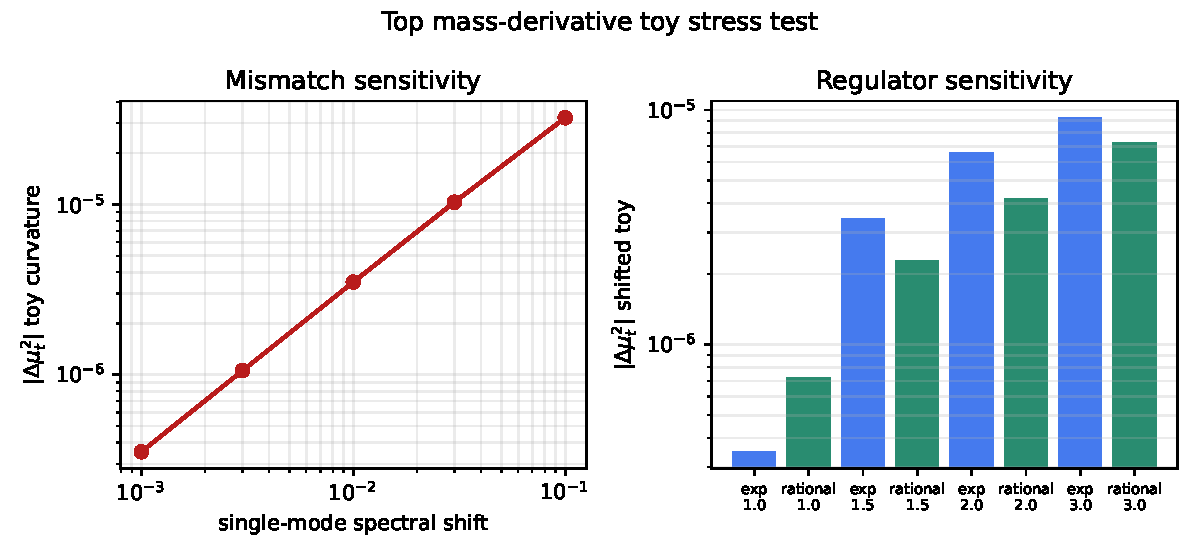
\includegraphics[width=0.86\linewidth]{figures/paper4_top_mass_derivative_toy_stress.pdf}
\caption{Toy mass-derivative stress test for the top determinant gate.  The
figure illustrates the required diagnostic behavior: same-domain paired spectra
remove the forbidden curvature, while a small spectral/domain mismatch leaves a
regulator-sensitive residue.}
\end{figure}

\section{What Is Reproduced And What Is Not}
The current package reproduces:
\begin{itemize}
\item a minimal $3+2$ stabilizer-compatible hypercharge direction;
\item conditional parent-selection gates linking two protected visible clusters, $\epsilon_3/\epsilon_2$ invariant roles, and the anomaly-safe target;
\item a conditional F1--F8 localization-forcing route for $\nu_i=\kappa_\tau^2|Y_i|$;
\item the Branch A working exponent $\nu_D=3/10$ once the $\nu_i=3|Y_i|/5$ rule is assumed;
\item the normalized $\operatorname{sech}^{3/10}$ zero mode;
\item the quartic overlap $I_4(3/10)=0.133756$;
\item an order-one parent-quartic requirement and a TeV-scale deformation estimate;
\item a sharpened statement of where the wall-$Q$ and top/Yukawa gates must enter.
\item a v0.2 single-package scaffold joining compact cell, wall domain,
same-domain regulator/product bookkeeping, and the $\epsilon_\tau$ scale gate;
\item the fixed dimensionless coefficient $y_t^{\rm parent}=0.9615522319$
inside that scaffold, before absolute-scale and matching closure.
\end{itemize}
It does not reproduce:
\begin{itemize}
\item the full Standard Model;
\item the Yukawa hierarchy;
\item the full parent-action derivation of the F1--F8 forcing conditions;
\item anomaly cancellation from a derived parent representation construction;
\item derivation of the $3\times2$ bridge and singlet/color channels from the parent action;
\item radiative stability;
\item the measured Higgs mass from a completed top determinant;
\item the top Yukawa strength or family hierarchy;
\item the absolute electroweak scale, because $\epsilon_\tau$, $C_A$, and the
compact-cell/wall embedding are not yet derived from the final parent action;
\item a collider-ready heavy-sector spectrum.
\end{itemize}

\section{Wolfram Language Audit}
The repository includes optional Wolfram Language audit scripts as an independent symbolic/numeric check of the formal skeleton:
\begin{itemize}
\item \texttt{Higgs\_Quartic\_Overlap\_Verification.wl} checks the normalized $\operatorname{sech}^\nu x$ profile, the quartic-overlap formula, $I_4(3/10)$, and the sensitivity range for the required parent quartic;
\item \texttt{BranchA\_Stabilizer\_Hypercharge\_Audit.wl} checks $\operatorname{Tr}T_\Sigma=0$, $\operatorname{Tr}T_\Sigma^2=1/2$, $\operatorname{Tr}T_Y^2=1/2$, and $T_\Sigma=-T_Y$, thereby verifying the stabilizer and hypercharge-normalization origin of the $3/5$ factor;
\item \texttt{G2\_Unoriented\_Line\_Quotient\_Audit.wl} checks that the line projector for $T_Y$ is invariant under $T_Y\mapsto -T_Y$, that $\operatorname{Tr}[(fT_Y)^2]=f^2/2$, and that the unit-line condition gives the two oriented representatives $f=\pm1$;
\item \texttt{Projection\_BRST\_Skeleton.wl} checks only the algebraic skeleton $s^2H=0$ and $Q_Dh_D=0$.
\item \texttt{Compact\_Gate\_Ledger\_Audit.wl} checks that the generated full-derivation ledger has continuous C0--C20 gate IDs, includes the C16/C17/C20 subgates, records the finite-residue and endpoint-matching gates, and keeps the claim boundary at proposition/program level rather than solved-proof level.
\end{itemize}
The generated log files are included in the reproducibility packet. These checks support the formula and algebra audit. They verify the normalization source of $3/5$, but they do not derive the localization postulate $\nu_i=\kappa_\tau^2|Y_i|$, prove anomaly freedom, prove regulator safety, or establish radiative stability.

\section{Why This Is Not Just Numerology}
The quartic-overlap calculation is evidence for internal coherence of the Branch A Higgs module, but not evidence for the full physical theory. The module becomes scientifically decisive only if the gates are passed in the right order: first derive the localization postulate that ties the exponent to $\kappa_\tau^2|Y_i|$, then prove the quotient/anomaly safety, then complete the top determinant, and only then compare the resulting heavy-sector predictions to collider constraints. Without those gates, the value $I_4(3/10)$ should be treated as a reproducible mechanism target rather than as physical validation.

\section{What Would Count As A Higgs-Sector Proof}
The proof target is stronger than the scaffold constructed in this manuscript.
It is the existence of a final parent action
\begin{equation}
S_{\rm parent}[\Psi]
\quad\Longrightarrow\quad
\text{Branch A gates}
\quad\Longrightarrow\quad
\text{SM-compatible Higgs sector},
\end{equation}
where the implication is dynamical rather than retrospective.  In particular,
$S_{\rm parent}$ would have to select the compact tau cell, the two protected
visible modules, the $3+2$ carrier, the hypercharge wall line, the BPS wall
profile, the same-domain $Q$/regulator package, and the scale unit
$\epsilon_\tau$ without using the measured Higgs mass, Higgs vev, or top mass.

Only after that would the remaining QFT tests become meaningful: anomaly
closure, regulator independence, Ward identities, top-determinant cancellation,
running/matching to the electroweak scale, and collider-compatible heavy-sector
predictions.  Thus the present result is not a Higgs proof.  It is a
paper-level reduction of the proof problem to a small number of explicitly
named gates.

\section{Remaining Proof Gates}
The present manuscript isolates the unresolved gates. These are not
presentation details; they are the conditions that separate the current
mechanism target from a Higgs-sector derivation.

\begin{enumerate}
\item \textbf{Explicit parent action and UV/continuum completion.} The v0.2
single-package action is a constrained scaffold, not the final microscopic
theory. A proof must define the parent configuration space, dynamical fields,
symmetry principle, measure, continuum limit, and admissible projection map
without using Higgs or top endpoints as inputs.
\item \textbf{Localization derivation.} The factor $3/5$ is now traced to
the Branch A hypercharge normalization, and the localization rule has been
sharpened into a conditional F1--F8 forcing route.  A completed proof must
still derive those F-conditions from the parent action: the two protected
visible modules, the unoriented hypercharge line/projector, the absence of
non-hypercharge leakage, the minimal BPS two-vacuum functional, and the
same-domain Hessian/$Q$ factorization.
\item \textbf{Parent-selection and representation derivation.} The current
packet narrows the $3+2$ carrier to a conditional chain of two protected
visible clusters, minimal $3+2$ support, $\epsilon_3/\epsilon_2$ invariant
roles, and an invariant/anomaly bridge. A proof must still derive those roles,
the $3\times2$ bridge, and the singlet/color channels from the parent
cohomology or Hessian structure rather than declaring an SM-like target.
\item \textbf{BRST/anomaly/regulator consistency.} The projection-BRST
skeleton explains how a quotient could protect the visible zero mode, but the
present packet checks only the algebraic skeleton. A proof must still define
the Hilbert-space domain, nilpotent charge, regulator, anomaly constraints, and
Ward identities. It must also show that these identities survive the same
continuum/UV completion used for the top determinant.
\item \textbf{Top determinant and radiative stability.} The top/flavor
deformation is still a roadmap calculation. The up-type top-sensitive slot and
same-domain wall-$Q$ pilot sharpen where the calculation must occur, but they
do not replace it. Until the physical determinant is computed, the Yukawa
strength is derived, and mismatch-independent or linear mass terms are shown to
be absent or quotient-trivial, the manuscript does not solve the Higgs
hierarchy problem. This is the decisive naturalness gate: a localized tree-level
quartic is not enough unless the radiative scalar-mass sensitivity is also
controlled.
\item \textbf{Compact tau-cell and scale.} The v0.2
single-package scaffold isolates the remaining absolute unit as
$\epsilon_\tau$ inside
$\Lambda_A=C_A\epsilon_\tau\mu_\tau({\cal K}_\tau)N_\tau\hat E_{\rm wall}$.
A proof must still specify the geometry/topology/spectral structure of
${\cal K}_\tau$, derive this universal parent density or stress-energy
scale, derive $C_A$, and show that the Branch A wall domain is induced from the
same compact tau cell rather than declared as a disconnected Higgs-sector
input. The most useful positive result would be a compact spectral or cell
geometry whose low-lying sector selects the $3+2$ stabilizer and whose defect
sector induces the hypercharge wall.
\item \textbf{Explicit compact-geometry v0.1.} The current v0.1 target is
the orbifold spectral package ${\cal K}_\tau=S^1/\mathbb Z_2$ with algebra
$(C^\infty({\cal K}_\tau)\otimes(M_3(\mathbb C)\oplus M_2(\mathbb C)))^{\mathbb Z_2}$,
Hilbert domain
$L^2({\cal K}_\tau)\otimes(\mathbb C^3\oplus\mathbb C^2)\otimes\mathbb C^2_{\rm wall}$,
and Dirac-like wall operator
$D_\tau=\sigma_1\partial_x+\sigma_2\kappa_\tau^2T_Yf(x)+D_{\rm gap}$.
A proof must still show that the self-adjoint orbifold domain, index residue,
positive-spectrum pairing, and regulator all come from this single package.
\item \textbf{Standard Model emergence.} A broader Branch A emergence program
must still derive the representation content, gauge dynamics, anomaly
cancellation, Yukawa pattern, and low-energy effective field theory from the
parent action. This paper contributes only a Higgs-module candidate gate.
\end{enumerate}

These gates make the status of the paper precise. The quartic-overlap result is
a reproducible and nontrivial mechanism target, but the localization,
cohomological consistency, and radiative-stability gates must all close before
the module can be promoted to a derivation.

\section{Compact Spectral Protection Program}
The technical companion keeps the full operator-domain ledger, but the main
paper needs the core logic explicitly.  The protection route is not merely a
localized wave-function ansatz.  It is the following compact spectral program:
\begin{equation}
\text{compact domain}
\rightarrow
Q\text{-paired self-adjoint operators}
\rightarrow
\text{index residue}
\rightarrow
\text{zeta-determinant cancellation}
\rightarrow
\text{allowed finite residues only} .
\end{equation}
The candidate compact geometry is the orbifold package
${\cal K}_\tau=S^1/\mathbb Z_2$ with a first-order wall operator $Q_\nu$.
The required domain theorem is:
\begin{equation}
Q_\nu:{\cal D}_-\to{\cal D}_+,\qquad
H_-=Q_\nu^\dagger Q_\nu,\qquad H_+=Q_\nu Q_\nu^\dagger ,
\end{equation}
with $H_\pm$ self-adjoint on one shared compact domain.  If this holds, then
for every positive eigenvalue $\lambda>0$ the map
\begin{equation}
\psi\mapsto \lambda^{-1/2}Q_\nu\psi
\end{equation}
pairs the positive spectra of $H_-$ and $H_+$ with equal multiplicity.  The
bulk positive-mode determinant then cancels at the zeta level, leaving only
kernel/index, anomaly/Ward, boundary, or frozen matching residues.

The negative status is equally important:
\begin{itemize}
\item a conditional compact spectral theorem is established only within the
stated operator-domain assumptions; the parent action has not yet selected the
required compact domain;
\item conditional positive-spectrum zeta-determinant cancellation follows
within the same-domain setup, and a physical top finite-residue extraction gate
is formulated, but the finite residue has not yet been computed from the parent
QFT;
\item same-domain anomaly/Ward and representation trace-cancellation gates are
formulated, but the parent-derived representation complex has not yet been
computed;
\item a UV/continuum admissibility criterion and microscopic completion target
are formulated, but no convergent parent action family is supplied;
\item a physical matching map and endpoint protocol are formulated, but no
numerical matching to the measured Higgs vev, top mass, or collider observables
has been performed.
\end{itemize}

This is why the compact spectral program is central to the paper.  Without it,
the construction is only a localization model.  With it, the Higgs-lightness
question becomes a sharply defined spectral problem: prove the self-adjoint
domain, prove positive-spectrum pairing, prove regulator/Ward compatibility,
and then compute the top-sensitive finite residue from the parent operator
family.

\section{Next Theorem Handoff}
The related structures in Section 2 are useful only if they sharpen the next
calculations.  The immediate handoff is:

\begin{center}
\begin{tabular}{p{0.25\linewidth}p{0.27\linewidth}p{0.34\linewidth}}
\toprule
\textbf{Open theorem} & \textbf{Best external toolkit} & \textbf{Concrete next deliverable}\\
\midrule
protected-form selection & cohomology and index theory & define the closure
and pairing complexes, prove which low-degree residues vanish, and isolate
$H^3_{\rm cl}$ and $H^2_{\rm pair}$ as first protected classes\\
compact spectrum & spectral geometry / self-adjoint extension theory & replace
the finite-box C9 pilot by a Q-paired compact $S^1/\mathbb Z_2$ domain and
compute or bound the spectrum\\
determinant finiteness & zeta determinant and heat-kernel methods & prove that
the same-domain positive spectra cancel up to zero-mode/index residue\\
quotient consistency & BRST cohomology and Ward identities & construct the
nilpotent charge, physical cohomology, anomaly test, and Ward identities on the
same domain\\
radiative stability & effective QFT matching & compute the top-sensitive
determinant and show whether mismatch-independent scalar mass terms are absent
or quotient-trivial\\
\bottomrule
\end{tabular}
\end{center}

This table is intentionally operational.  A future paper can close one row
without claiming the whole Higgs sector.  The strongest next target is the
protected-form selection row, because it would turn the $3+2$ carrier from a
minimal candidate into a parent-selected algebraic consequence.

\section{Claim-Upgrade Ladder}
The manuscript should be read with the following claim ladder.  Each level
licenses only the next stronger statement after the listed gate is closed.

\begin{center}
\begin{tabular}{p{0.24\linewidth}p{0.33\linewidth}p{0.29\linewidth}}
\toprule
\textbf{Closed gate} & \textbf{Allowed claim} & \textbf{Still forbidden}\\
\midrule
quartic overlap only & reproducible mechanism target & Higgs derivation or
naturalness solution\\
localization rule derived & Branch A maps Higgs quartic to an order-one parent
coupling & Standard Model derivation\\
protected-form/index selection & $3+2$ carrier becomes parent-selected rather
than postulated & full gauge/Yukawa sector\\
shared compact spectrum and C18 pairing & positive-spectrum cancellation target
becomes theorem-level & physical radiative stability\\
C19--C20 determinant residue admitted & determinant route becomes regulator-safe
candidate & measured Higgs/top masses\\
top determinant and matching closed & Higgs-lightness mechanism can be claimed
within Branch A & full Tau Core or TOE validation\\
\bottomrule
\end{tabular}
\end{center}

At the present stage the paper sits at the first level and partially organizes
the next levels.  It does not yet license the later claims.

\section{Near-Term Falsifiable Prediction}
The current module predicts a narrow kind of future test rather than an already validated signal. If the top/flavor deformation gate is completed with a natural spurion $\delta_\star\sim10^{-3}$, the same equations imply a parent scale $M_\tau$ in the multi-TeV range and a Higgs-sector spectral threshold
\begin{equation}
m_{\rm gap}\simeq\nu_D M_\tau \sim 2\text{--}4\,{\rm TeV}.
\end{equation}
The associated Higgs-coupling deviations should be parametrically of order
\begin{equation}
\frac{\Delta g}{g}\sim\frac{v^2}{m_{\rm gap}^{2}}\sim10^{-3}\text{--}10^{-2} .
\end{equation}
This is a falsifiable target, not a confirmed prediction. The module weakens if the completed determinant forces much larger deviations, no TeV-sector threshold, or collider-excluded states.

\section{Validation Gates}
The module would fail if any of the following gates fail:
\begin{itemize}
\item the Branch A projection metric rule $\nu_i=3|Y_i|/5$ cannot be forced from the parent action or the F1--F8 sufficient conditions fail;
\item the two-block / $3+2$ / invariant-role chain cannot be derived from the parent action or stability structure;
\item the $3\times2$ bridge and anomaly-safe visible target cannot be obtained without post-hoc representation choice;
\item the physical $Q_\mu$ operator cannot be derived from the same wall-Hessian/domain package;
\item the parent quartic is not canonical or requires large tuning;
\item the projection-BRST quotient is anomalous or regulator-dependent;
\item a visible Higgs mass is unavoidable at $\delta_\star=0$;
\item the top determinant produces a large mismatch-independent or linear mass term, or requires an inserted Yukawa hierarchy;
\item $\epsilon_\tau$, $C_A$, or the wall-cell embedding must be chosen from
the measured Higgs vev or top mass;
\item the TeV-sector spectral window is excluded by Higgs coupling or direct-search constraints.
\end{itemize}

% BEGIN OBSERVER UPDATE 20260914
\section{Observer realization: inherited results and physical boundary}
\label{sec:observer-update-20260914}
The current observer programme distinguishes a conditional mathematical
construction from an occupied physical measuring system. The source order
remains base plus one universal seed, stabilized morphological response,
observer--source restriction, shared descriptor, and resolved terminal
readouts. Neither a detector nor an empirical residual constructs the parent
body backwards. Dynamics below concern downstream subsystems only.

The canonical observer-origin derivation, Sections 22--26, owns the following
results. The existing joint source action fixes static and frequency-dependent
response together. Variation of the BRAC potential couples to the field
square; a linear field coupling is a distinct comparator unless derived by
expansion about an occupied background. Fixed canonical means select a unique
coherent state in a finite positive harmonic packet only if there is no excess
fluctuation energy. This is a free/asymptotic preparation statement, not the
ground state of an interacting detector. For the existing coupled harmonic
pair, the joint ground is pure but either local subsystem is mixed, with its
covariance fixed by the complete joint Hamiltonian.

These are conditional derivations and internal numerical checks. The actual
observer--source context, physical preparation process, kinetic/energy
calibration and stable operational resolution remain unproved. The existing
ORA-T1 selector conditionally chooses stable quantizers when the occupied
context, admissible partition family and positive closure barrier are supplied;
it does not establish those physical premises. A computed ground state is not
a preparation mechanism, and a covariance or optimal abstract measurement is
not an implemented stable quantizer $Q_{OS}$.

\paragraph{Ownership and use.}
The central observer-origin note owns the new contact, state and covariance
derivations; the body-readout technical companion carries the consolidated
mathematics. Foundation Papers IV, V and VI retain physical-selection,
clock-descent and quantum-readout ownership, respectively. This paper imports
only the consequences within its scope. No observational dataset, baseline,
frozen coefficient, score or empirical conclusion is revised by this update.
The reproducibility supplement records the source hashes and the exact
conditional/physical distinction.


\paragraph{Consequence for this paper.}
These results do not select a particle spectrum, coupling constant, Higgs vacuum or gravitational terminal. Common source ancestry remains weaker than physical realization of those sectors.
% END OBSERVER UPDATE 20260914

% BEGIN STATE UPDATE 20260918
\section{Source identification and recovery}
The current observer audit separates a conditional forward construction from physical source selection. A frozen body, occupied observer incidence, preparation, complete instrument and stable resolution can determine records without selecting those inputs from Nature. Equal effects do not fix postmeasurement states, and symmetry within a chosen interaction family does not exclude other symmetric couplings. These results do not select a particle spectrum, coupling constant, Higgs vacuum or gravitational terminal. Common source ancestry remains weaker than physical realization of those sectors.

\paragraph{Dependency and claim ownership.}
Foundation VI and the body--readout technical companion own the finite instrument/access proof; Foundation IV and TD-0 retain physical source selection; Foundation V, the temporal synthesis and seed--body companion own the gradient/inertial distinction. This paper inherits only the stated specialization. Canonical assumptions, countermodels and calibration audits are in \url{https://github.com/tau-core-research/tau-core-theory/blob/main/docs/tau_rqm_instrument_to_record_bridge_001.md}. No physical seed, Nature occupation or Tau-exclusive observation is established by this update. Existing empirical endpoint definitions and scores are unchanged.
% END STATE UPDATE 20260918

\section{Conclusion}
The Branch A Higgs module links a $3+2$ stabilizer, hypercharge normalization,
a $\operatorname{sech}^{3/10}$ visible zero mode, and a quartic overlap
requiring an order-one parent quartic. The paper establishes a compact,
reproducible mechanism target: if the Branch A localization rule is derived,
the Higgs quartic is mapped to a natural parent-scale coupling rather than an
extreme hierarchy. The hard blockers are now sharply identified: an explicit
final parent action, continuum/UV completion, a concrete compact tau-cell
geometry, QFT-level BRST/anomaly/regulator closure, top-determinant radiative
stability, and physical matching. The manuscript still does not establish the
full parent theory, the measured Higgs vev, the measured top mass, the Standard
Model, or the Higgs hierarchy solution. The present result is a mechanism
target and spectral proof program, not a completed Higgs-sector derivation.

\bibliographystyle{plain}
\bibliography{references}
\end{document}
